\documentclass[margin,line]{resume}
\usepackage[defblank]{paralist}
\usepackage{pdfpages}
\usepackage{blfootnote}
\setdefaultitem{\tiny \textbullet}{}{}{}{}{}
\setdefaultleftmargin{0em}{}{}{}{}{}
\begin{document}
\name{\Large Russell E. Harmon}
\begin{resume}

\section{\mysidestyle Contact \\ Information}\vspace{2mm}
	\begin{asparablank}
		\item Rochester Institute of Technology \hfill 2710 Avenue J NW
		\item 39 Nathaniel Rochester Hall \hfill Winter Haven, FL 33881
		\item Rochester, NY 14623 \hfill russ@eatnumber1.com
		\item (863) 514-7014 \hfill blog.eatnumber1.com
	\end{asparablank}

\section{\mysidestyle Education}
		\begin{compactdesc}
			\item[Rochester Institute of Technology] \hfill {\footnotesize 2006 - Present}
			\begin{compactitem}
				\item {\small Computer Science BS/MS}
				\item {\small Music minor}
			\end{compactitem}
			\item[Herbert H. Lehman High School] - College Prep Program \hfill
			{\footnotesize 2002 - 2006}
			\item[Lehman College] - Course work in Q-Basic (age 12)
		\end{compactdesc}

\section{\mysidestyle Experience}
	\begin{compactdesc}
		\item[SafeNet Inc] - Belcamp, MD \hfill {\small June 2008 - Present}
		\\* Engineering Intern \hfill {\footnotesize http://www.safenet-inc.com}
		\begin{compactitem}
			\item {\small Working as a developer on a team of 7 on SMCII (the
			SafeNet Management Console)}
			\item {\small Java development with JBoss, Hibernate and JSF}
		\end{compactitem}
		\item[New York City Department of Education] - Bronx, NY \hfill
		{\small September 2002 - June 2006}
		\\* IT Specialist \hfill {\footnotesize http://schools.nyc.gov}
		\begin{compactitem}
			\item {\small Setup and maintain computer systems throughout Lehman
			High School}
			\item {\small Diagnose, repair, and maintain the network}
			\item {\small Diagnose and eliminate viruses and malware on the
			school's network and computer systems}
			\item {\small Audit the network for malicious activity}
		\end{compactitem}

		\item[New York Sailing \& Yacht Club] - Bronx, NY \hfill {\small
		2001-2005}
		\\* Launch Operator \hfill {\footnotesize http://www.startsailing.com}
		\begin{compactitem}
			\item {\small Taxi patrons to their boats moored in the harbor}
			\item {\small Small craft operation - experienced in motor and sail
			boats}
		\end{compactitem}

		\item[City Island Computer Services] - Bronx, NY \hfill {\small
		1998-1999}
		\\* Apprentice (age 10)
	\end{compactdesc}

\section{\mysidestyle Technical Skills}
	\begin{asparablank}
		\item UNIX/bash
		\item Java
		\item C/C++
		\item PC troubleshooting and repair
	 \end{asparablank}

\section{\mysidestyle Honors \& Awards}
	\begin{asparablank}
		\item NYC Regional Robotics Award winner
		\begin{compactitem}
			\item {\small 27th place in the national competition}
		\end{compactitem}
		\item Honor Roll 2003-2005
		\item Visual Basic Programming Award for academic excellence 2005
		\item First Place Sailing Award 2000, 2002
	\end{asparablank}

\section{\mysidestyle Special Accomplishments}
	\begin{asparablank}
		\item At age 8, built my first computer. At age 12, attended my first
		programming class at Lehman College.
		\item Designed and implemented an encryption algorithm using a
		combination of transposition and substitution.
		\item Community Service - built a boat for needy children from the South
		Bronx.
	\end{asparablank}

\section{\mysidestyle Personal \\ Strengths}
	\begin{asparablank}
		\item Ingenuity
		\item Thinking Outside the Box
		\item Perseverance
		\item Motivated to Excel
	\end{asparablank}

\section{\mysidestyle Certifications}
	\begin{asparablank}
		\item Cisco Academy, with honors (terms 1 and 2)
		\item A+
		\item MOUS (Word)
	\end{asparablank}

\blfootnote{References available on request.}
\end{resume}
\pagebreak[4] % The 4 makes it a VERY INSISTENT requirement for a page break.
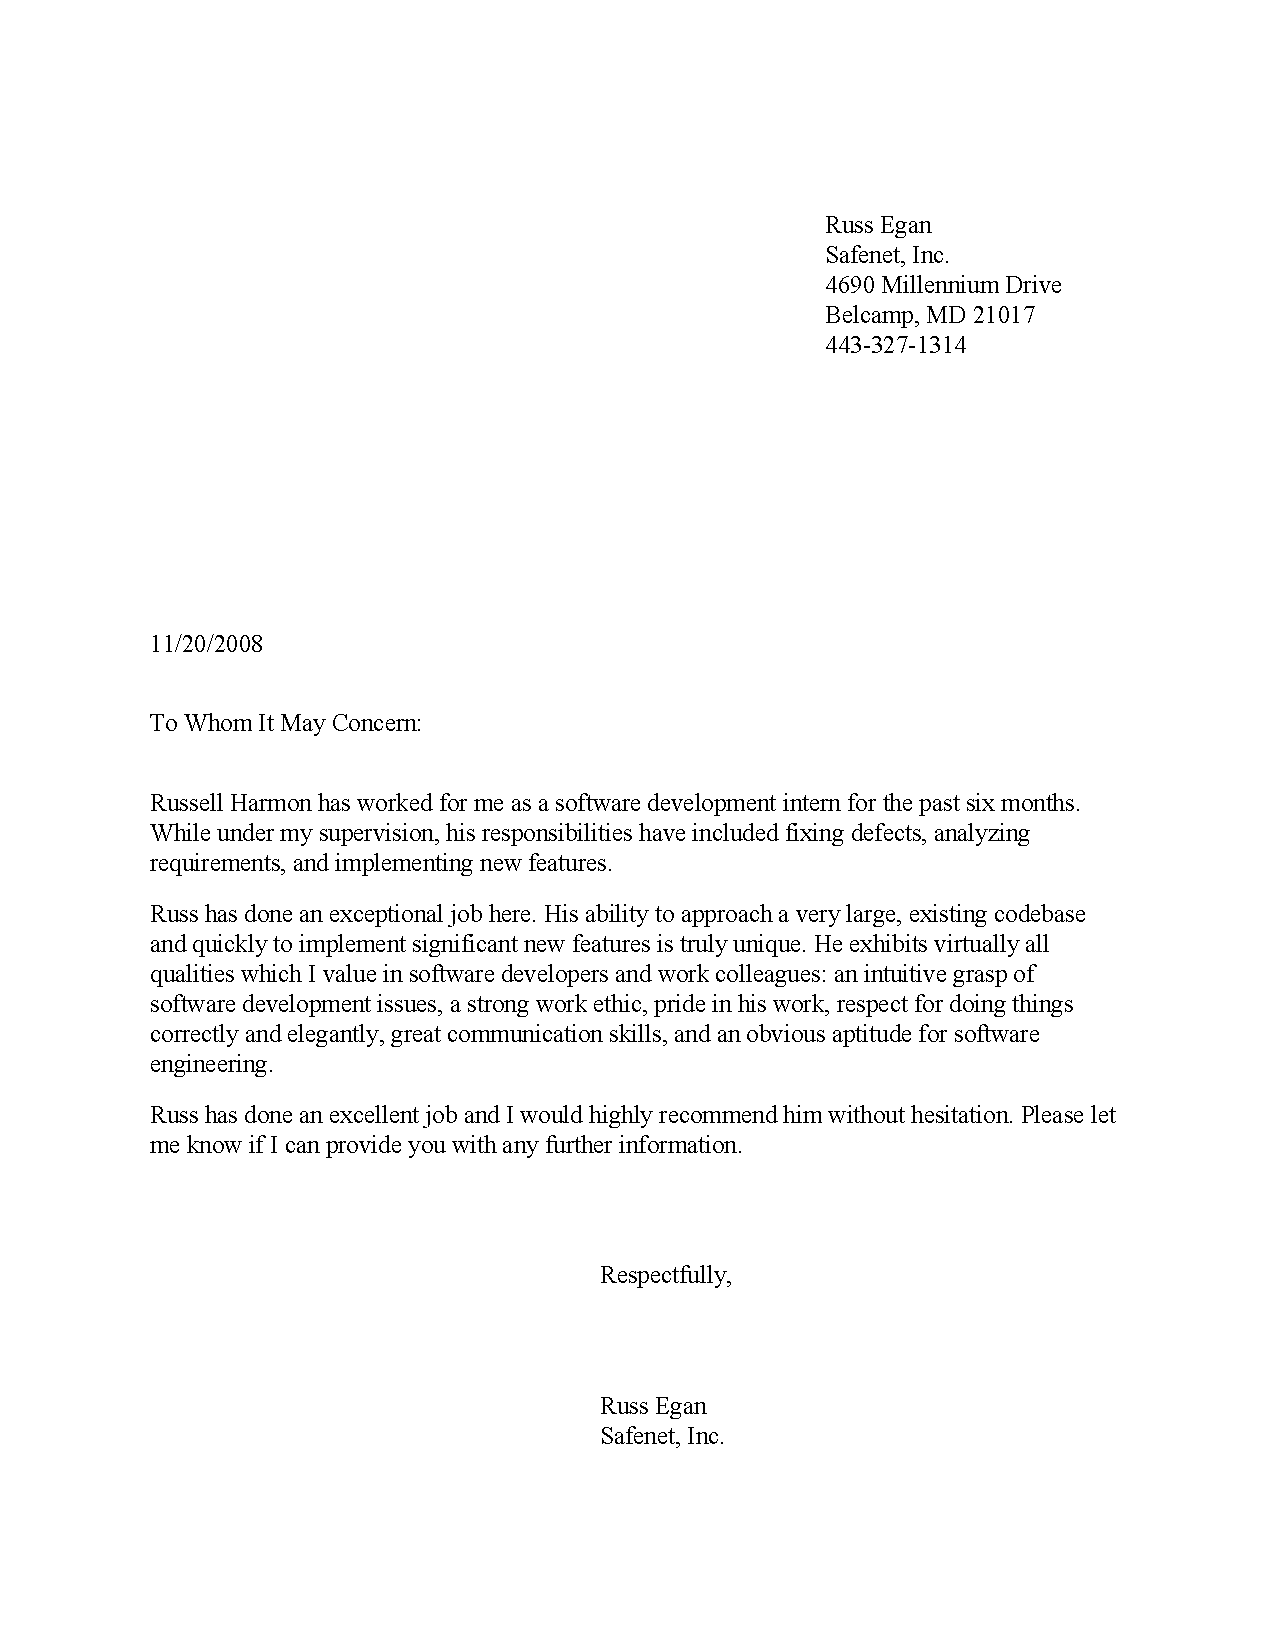
\includepdf[offset=-94 0,pages=1]{sfnt-recommendation}
\end{document}
